\section{Motivating Example}
\label{sec:motivation}

\begin{figure*}[ht]
    \centering
    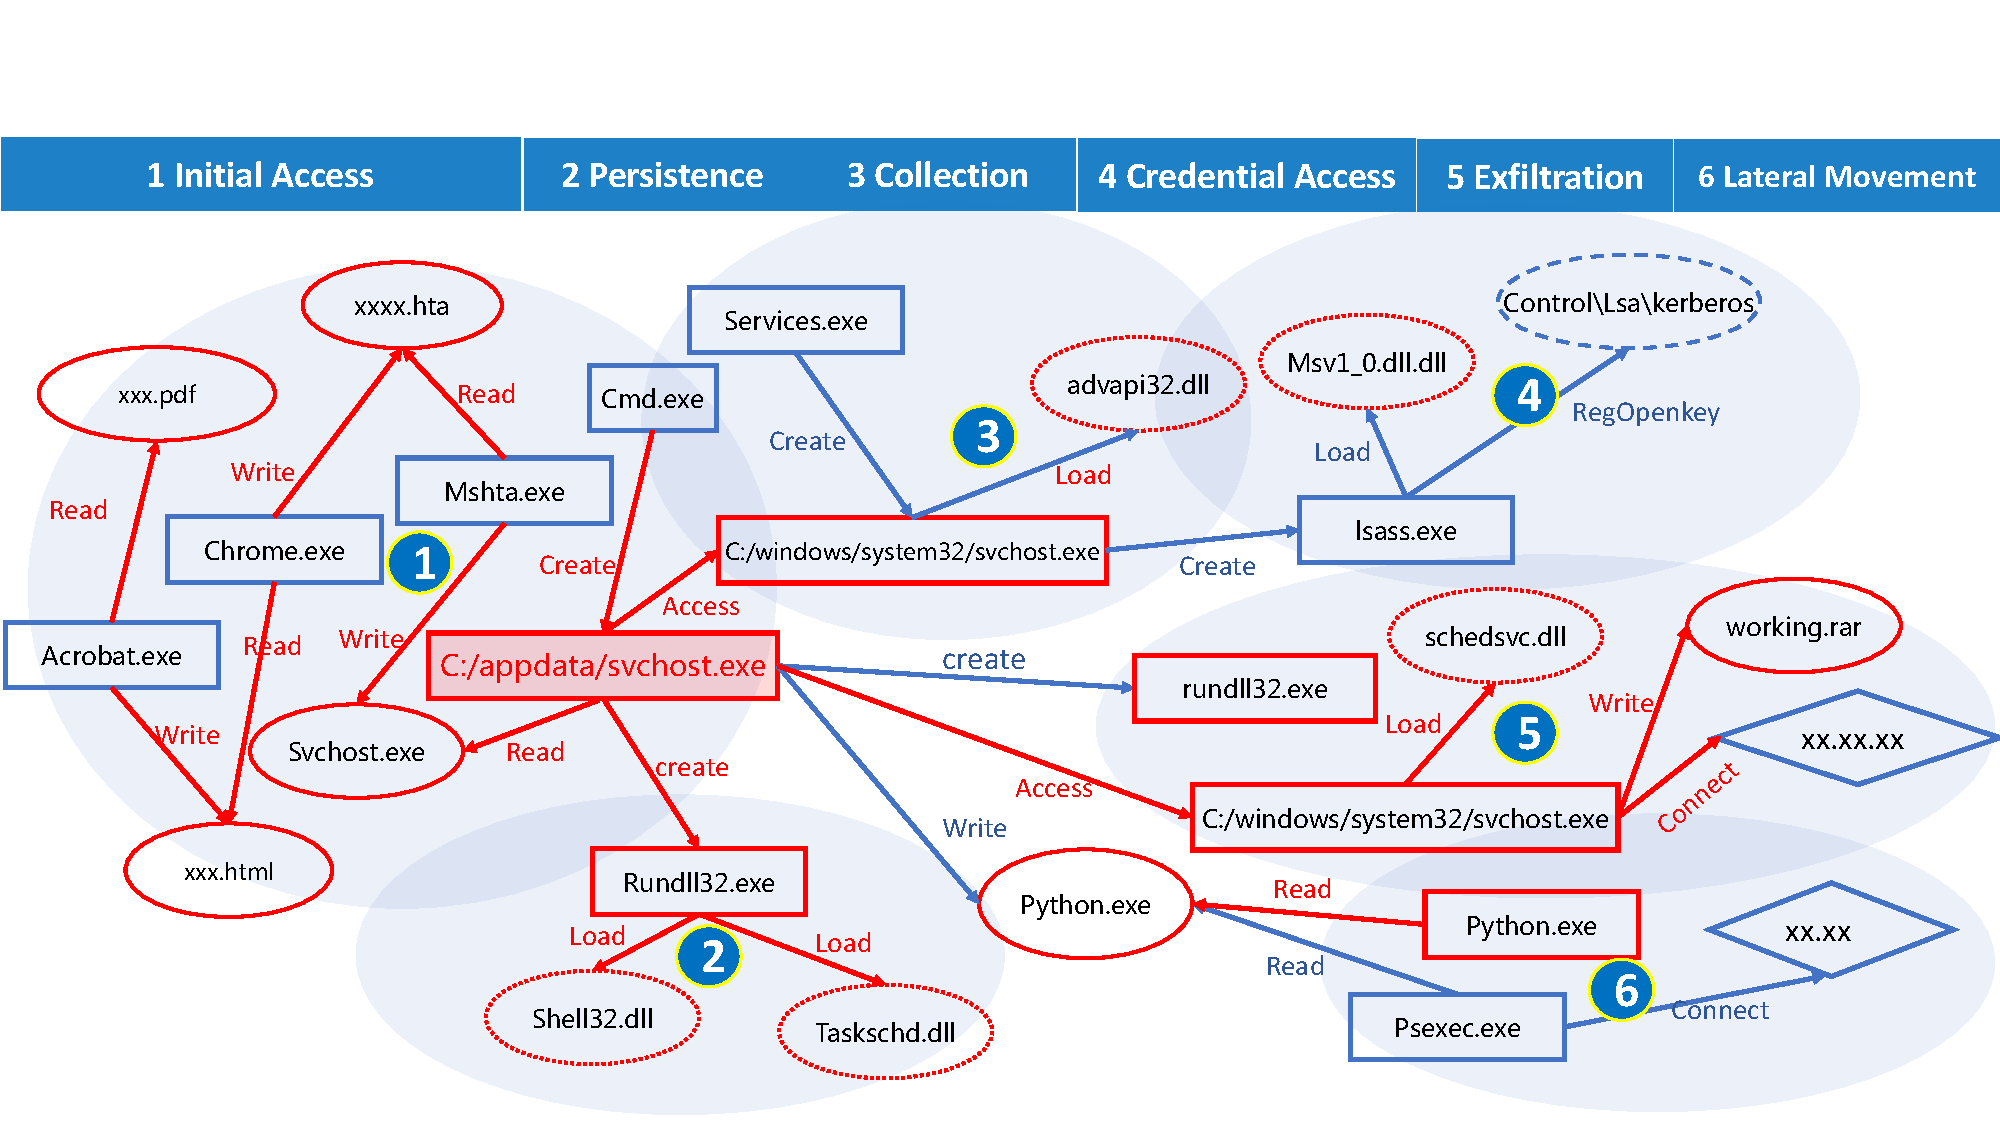
\includegraphics[width=0.9\textwidth]{figs/example.pdf}
    \caption{ 
    System entities are represented by nodes in the graph. 
    The attack-relevant elements are highlighted in red, while those representing regular events and nodes are displayed in blue.
    Processes, file-type entities (dlls, registry, files, etc.), and sockets are represented by rectangles, ovals, and diamonds. Solid line ovals represent files, dashed line ovals represent registries, and dotted line ovals represent DLLs. A series of operations is represented by an edge, such as read, create, and load. We have segmented the attack progression into six distinct steps using a light blue backdrop. }
    \label{fig-example}
    \end{figure*}

\paragraph{Attack Scenario}
Figure~\ref{fig-example} illustrates a simplified provenance graph derived from audit records of a trojan-induced APT attack. System entities are represented by nodes in the graph. 
Processes, file-type entities (dlls, registry, files, etc.), and sockets are represented by rectangles, ovals, and diamonds. Solid line ovals represent files, dashed line ovals represent registries, and dotted line ovals represent DLLs.
A series of operations is represented by an edge, such as read, create, and load.
There are 6 steps that are followed in the trojan-induced APT attack.
%In our analysis of APT attack reports \cite{eclecticiq2023,microsoft2023,paloaltonetworks2023}, we identify common attack steps and stealthy methods, such as Process Masquerade, Process Injection, Process Hollow, and DLL-Side Loading\cite{eclecticiq2023}. As a result of the use of four common obfuscation techniques, we were able to assemble ten scenarios for APT attacks using 23 malicious functions disguised as DLLs and program names.
%One of attack scenario as motivating example is used to illustrate current detection methods' limitations as well as our approach's intuition.


\begin{enumerate}[leftmargin=*]
    \item Initial Access: The attacker first sends the victim a malicious pdf file \textit{xxx.pdf} that contains a virus. Unfortunately, the application \textit{Acrobat.exe} that reads PDF files does not protect against the malicious code that is hidden inside the document. As a result, the malicious code downloads the malicious \textit{xxxx.hta} file, and the malicious program \textit{svchost.exe} is then downloaded and executed within the directory \textit{c:/appdata/svchost.exe}.
    \item Persistence: As an attempt to hide itself, this malicious \\ \textit{C:/appdata/svchost.exe} opens \textit{rundll32.exe}, which then uses a DLL Side-Loading technique to load a malicious DLL \textit{shell32.dll}, which contains functionality for establishing persistence in the compromised system.
    \item Collection: Malicious \textit{C:/appdata/svchost.exe} then injects malicious \textit{advapi32.dll} processes into a benign \\ \textit{C:/windows/system32/svchost.exe} and uses the malicious dll disguised as \textit{advapi32.dll} to gather information.
    \item Credential Access: Meanwhile, by exploiting a vulnerability, the attackers downgraded Kerberos to the more vulnerable NTLM protocol (\textit{Msv1\_0.dll}). In order to move lateral within the network, they stole credentials from the domain.
    \item Exfiltration: A malicious attacker hollows out a portion of the memory space of the benign process svchost, fills it with malicious programs, and packages up the information into a ZIP file known as \textit{working.rar}.
    \item Lateral movement: After obtaining the credentials from step 4, the attacker executed the renamed \textit{python.exe} file, thus gaining lateral access to the network.
\end{enumerate}




%\paragraph{Challenges to Existing Solutions}
%Our simulated APT attack shows the following limitations of provenance-based threat detection:
%\begin{itemize}[leftmargin=*]
%    \item \textit{Misuse-based Detection}:  A misuse-based detector\cite{milajerdi2019holmes,milajerdi2019poirot} detects cyber threats by matching audit records with security policies that describe attack semantics. The creation of these security policies is time-consuming and requires domain knowledge, even though such detection maintains a low false-positive rate. As shown in our example, a single TTP can correspond to a variety of different attacks, while "initial access" can be implemented in a variety of ways, our case utilizing \textit{Mshta.exe}. It is the responsibility of experts to cover all attack behaviors for a given TTP, but this is a time-consuming and labor-intensive process, and it cannot handle unknown or evolving threats. In addition, experts' subjective interpretations of attacks, varying proficiency levels, or even human error can affect the quality of policy formulation.
%    \item \textit{Anomaly-based Detection}: Anomaly-based detection techniques detect deviations, but they rarely provide a deeper understanding of the underlying attack mechanisms. Identifying the root cause of this attack scenario can be difficult due to the deluge of records generated by this attack scenario. As an example, Unicorn\cite{han2020unicorn} may trigger alerts across a graph, but it cannot pinpoint which particular entities or patterns are triggered. As a result of their ability to mimic benign activities, they are practically imperceptible, and in this attack scenario, many disguised behaviors can be seen. Process hollow is one of the disguised behaviors used in step 5. We get \textit{rundll32.exe} and the malicious \textit{svchost.exe} using the same vector based on Shadewatcher\cite{zengy2022shadewatcher}, so we cannot detect exceptions. Furthermore, the number of anomalous entries in benign logs is very low (less than 1\% of all entries are malicious). The limited representation of stealthy threats in logs makes it difficult to train a robust and reliable model.
%    \item \textit{Statistics-based Detection}: Even though statistics-based approaches \cite{liu2018towards,hassan2019nodoze,hassan2020we} identify potential threats within graphs, they often misinterpret benign but rare threats. For instance, in our motivating example, svchost has many functions, one of which hosts the schedule service. False alarms can occur due to infrequent incidents being flagged as attacks.
%\end{itemize}
%All of these methods have difficulties in identifying attacks in a timely and accurate manner. Further, they do not provide sufficient granularity to clarify and explain specific attack behaviors, which complicates the identification and response process in the event of an attack.



\paragraph{Our Solution}
\label{sec:intuition}
%As we mentioned previously, we analyze numerous APT attack
%reports\cite{eclecticiq2023,microsoft2023,paloaltonetworks2023} and discovered that attackers often employ disguise techniques to hide their malicious activities.
%The techniques include Process Masquerade, Process Injection, Process Hollow, and Direct Loading.
%It is generally true that as attackers progress from straightforward masquerading techniques, like mimicking legitimate processes, to more sophisticated ones, such as DLL\-side loading, the stealthiness of their disguises tends to increase.

In spite of the masquerading method, there are inherent behavioral invariant associated with genuine program behavior, regardless of the disguised method - execution paths, parent-child relationships, permissions, as a process must execute operations, some of which must be performed in sequence, etc.
To capture such constraints, we define behavioral invariants (see Section~\ref{sec:toolDefs} for more details) to limit the genuine program behaviors.
% Specifically, the behavioral invariants considered in this work are defined in Section~\ref{sec:toolDefs}:

% \fbox{
% \linyun{TODO: $p_1 \land p_2 \land ... $}
% }

However, there were significant deviations from these behavioral invariants. 
While \textit{svchost.exe} is typically spawned by \textit{services.exe}, the malicious variant here is spawned by \textit{cmd.exe}. Additionally, its execution path was not what one might expect for an authentic \textit{svchost.exe}.
For more stealth attacks, like process injection as shown in step 3, a maliciously injected \textit{advapi32.dll} disrupts the expected sequence of events and violates the associated constraints. Thus, it is essential that profiles and constraints are taken into account as detection signals for regular processes in order to improve detection capabilities.


% \fbox{
% \linyun{TODO:  $p_1 \land p_2 \land ... \land q_1$}
% }

% \linyun{$q_1$ for the runtime behaviors}

